\section{Results}\label{sec:results}

All scores in this section are on the reference set (Section~\ref{sec:ref}): \NRefSpecs{}
held-out official specifications, \NRefInScope{} of them in scope. Weighted accuracy is
$\mathrm{acc}_w$ of equation~\eqref{eq:accw} under the equal split; brackets give
\CfgCI\% intervals from \NBoot{} stratified bootstrap resamples. The NNLS split is reported
where it changes a conclusion.

\subsection{RQ1: cross-lingual transfer and the value of official labels}\label{sec:rq1}

\textbf{Answer.} Transfer from non-Thai products does most of the work. An \NameEfive{} MLP
trained only on non-Thai products classifies \AccWEfiveMLPZeroShot\%
[\AccWEfiveMLPZeroShotLo, \AccWEfiveMLPZeroShotHi] of the evaluated CPI weight correctly.
Thai weak labels add nothing, budgets of up to \CfgBudgetMax{} official labels add little,
and all \NMocTrainval{} official labels raise it to \AccWEfiveMLP\%
[\AccWEfiveMLPLo, \AccWEfiveMLPHi].

Figure~\ref{fig:learning} traces the learning curve. With Thai weak labels added the score is
\AccWEfiveMLPThaiWeak\%; with \CfgBudgetMax{} official labels on top of the weak ones it is
\AccWEfiveMLPPlusThousand\%. Only the full official set moves it clearly: the paired gain of
all official labels over zero-shot transfer is \DiffEfiveMLPEfiveMLPZeroShot{} percentage
points [\DiffEfiveMLPEfiveMLPZeroShotLo, \DiffEfiveMLPEfiveMLPZeroShotHi]. That gain depends on
how the weight is spread inside the official cells: under the NNLS split it is
\DiffEfiveMLPEfiveMLPZeroShotNnls{} points [\DiffEfiveMLPEfiveMLPZeroShotNnlsLo,
\DiffEfiveMLPEfiveMLPZeroShotNnlsHi], and the interval includes zero. Official labels on their
own need the whole set: with \CfgBudgetMax{} of them the classifier reaches only
\AccWEfiveMLPMocThousand\%, and with all of them \AccWEfiveMLPMocOnly\%. The
other encoders tell the same story at lower levels: zero-shot \NameBge{} MLP reaches
\AccWBgeMLPZeroShot\% and the zero-shot fine-tuned XLM-R \AccWXlmrFTZeroShot\%; with every
label the three are within a few points of one another (\AccWEfiveMLP\%, \AccWBgeMLP\% and
\AccWXlmrFT\%).

\begin{figure}[t]
\centering
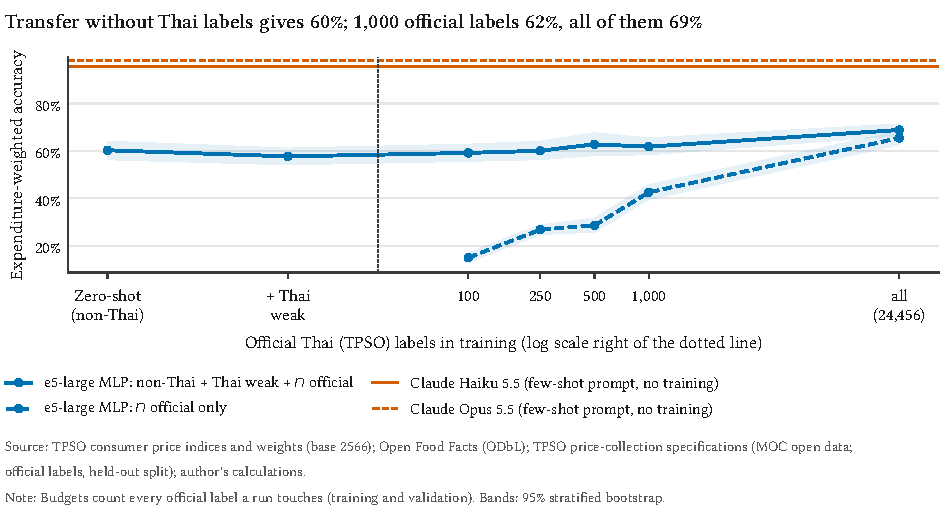
\includegraphics[width=\textwidth]{fig05_learning_curve.pdf}
\caption{\textbf{Transfer from non-Thai products gives \AccWEfiveMLPZeroShot\% weighted
accuracy with no Thai label; \CfgBudgetMax{} official labels give \AccWEfiveMLPPlusThousand\%
and all of them \AccWEfiveMLP\%.} \NameEfive{} MLP by training pool: zero-shot (non-Thai weak
labels), plus Thai weak labels, plus $n$ official labels (solid), and $n$ official labels
alone (dashed). Horizontal lines: the two LLMs, prompted with \CfgFewShot{} official examples
per item. Bands: \CfgCI\% stratified bootstrap. Source: Open Food Facts; MOC; TPSO; author's
calculations.}
\label{fig:learning}
\end{figure}

Plain accuracy hides all of this. The held-out list is mostly out-of-scope
specifications, and a classifier that answers \textsc{oos} to almost everything scores well
on it: the \NameEfive{} MLP trained on a hundred official labels alone is right on
\AccEfiveMLPMocHundred\% of the list but on only \AccWEfiveMLPMocHundred\% of the evaluated
CPI weight. Conversely, the zero-shot classifier is right on only \AccEfiveMLPZeroShot\% of
the list because it was never shown an out-of-scope Thai text, yet it measures most of the
weight correctly. A metric weighted by expenditure is not a refinement here; it reverses the
ranking.

The input fields matter less than the labels. Dropping the brand from the input costs
\DiffEfiveMLPEfiveMLPNoBrand{} points [\DiffEfiveMLPEfiveMLPNoBrandLo,
\DiffEfiveMLPEfiveMLPNoBrandHi]; dropping the quantity costs nothing measurable
(\DiffEfiveMLPEfiveMLPNoQty{} [\DiffEfiveMLPEfiveMLPNoQtyLo, \DiffEfiveMLPEfiveMLPNoQtyHi]).
Figure~\ref{fig:alignment} shows why transfer works for some items and not for others: in
the embedding space, Thai beverages, eggs and dairy products sit among non-Thai products of
the same item, while Thai processed seafood, processed meat and fresh fruit do not.

\begin{figure}[t]
\centering
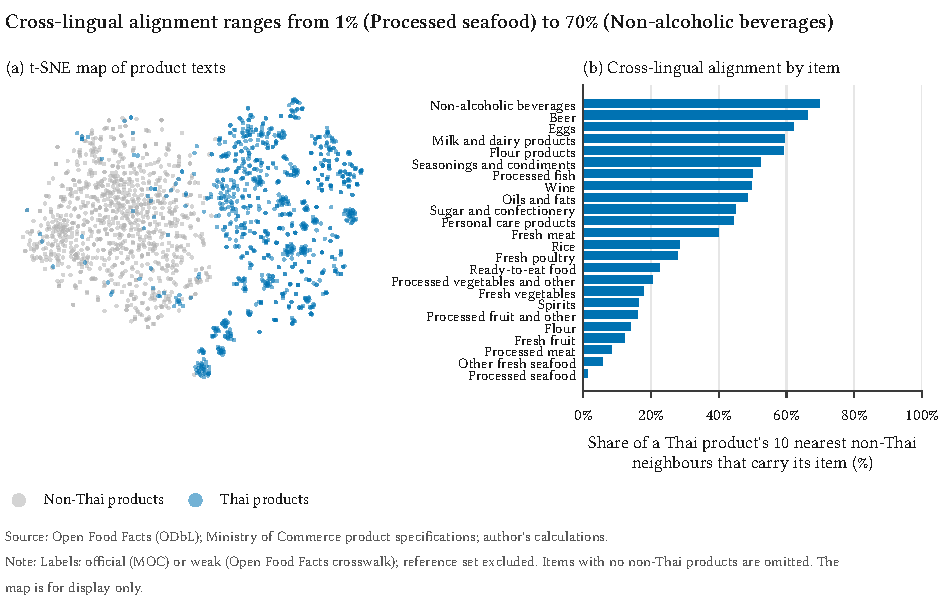
\includegraphics[width=\textwidth]{fig08_embedding_map.pdf}
\caption{\textbf{Thai products sit next to non-Thai products of the same item for some items
and not for others.} (a) t-SNE map of a balanced sample of product texts (display only).
(b) Cross-lingual alignment: the share of a Thai product's \CfgAlignK{} nearest non-Thai
neighbours, in the full \NameEfive{} space, that carry its item. The reference set is
excluded. Source: Open Food Facts; MOC; author's calculations.}
\label{fig:alignment}
\end{figure}

\subsection{RQ2: accuracy, coverage and cost}\label{sec:rq2}

\textbf{Answer.} On official Thai text the LLMs are far ahead.
\NameOpus{} classifies \AccWOpus\% [\AccWOpusLo, \AccWOpusHi] of the evaluated weight correctly
and \NameHaiku{} \AccWHaiku\% [\AccWHaikuLo, \AccWHaikuHi], against \AccWXlmrFT\% for the best
cheap method. A cascade that sends the \NameEfive{} MLP's unsure products to \NameOpus{}
matches \NameOpus{} at \CostPctCasEfiveMLPOpus\% of its cost.

The gap between the LLMs and every cheap method is large and certain: \NameHaiku{} is ahead
of the \NameEfive{} MLP by \DiffHaikuEfiveMLP{} points [\DiffHaikuEfiveMLPLo,
\DiffHaikuEfiveMLPHi], of \NameBge{} by \DiffHaikuBgeMLP{} and of the fine-tuned XLM-R by
\DiffHaikuXlmrFT. \NameOpus{} is ahead of \NameHaiku{} by \DiffOpusHaiku{} points
[\DiffOpusHaikuLo, \DiffOpusHaikuHi] and costs \CostRatioOpusHaiku{} times as much: USD
\CostOpus{} per million products against USD \CostHaiku{}, while the embedding classifiers
cost well under a dollar (USD \CostEfiveMLP{} for the \NameEfive{} MLP;
Figure~\ref{fig:cost}). Under the NNLS split every score falls, because NNLS moves weight
onto the item with the largest LLM error (below), but the ranking does not change
(\NameOpus{} \AccWOpusNnls\%, \NameHaiku{} \AccWHaikuNnls\%, \NameEfive{} MLP
\AccWEfiveMLPNnls\%).

\begin{figure}[t]
\centering
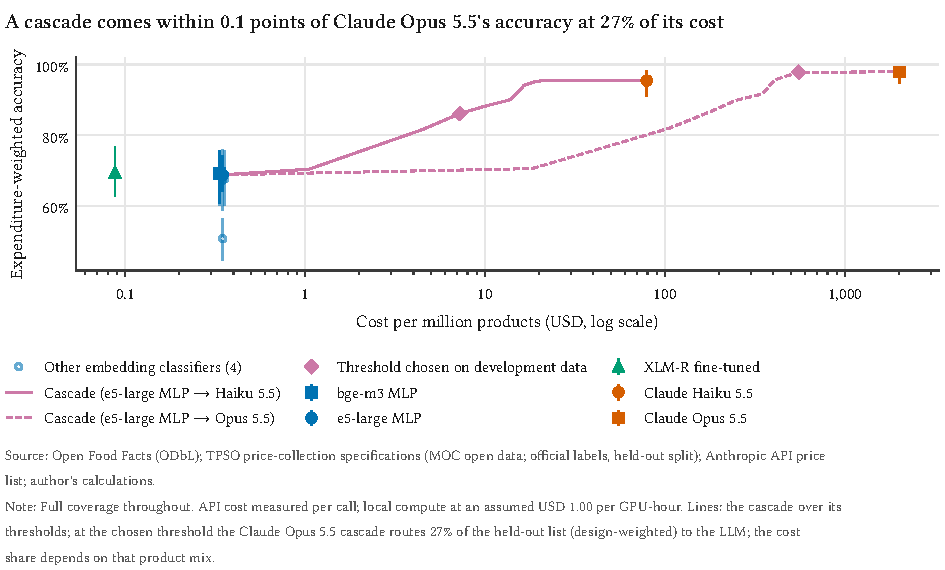
\includegraphics[width=\textwidth]{fig04_cost.pdf}
\caption{\textbf{A cascade from the \NameEfive{} MLP to \NameOpus{} matches \NameOpus{} at
\CostPctCasEfiveMLPOpus\% of its cost; no cheap method comes close to either LLM.} Weighted
accuracy at full coverage against cost per million products (log scale). Lines: each cascade
over its candidate thresholds; diamonds: the threshold chosen on development data. API cost
measured per call; local compute at an assumed USD~\CfgGpuUSDHour{} per GPU-hour. Source:
Open Food Facts; MOC; TPSO; Anthropic API price list; author's calculations.}
\label{fig:cost}
\end{figure}

Cascades work when the threshold is set where the cheap model is reliable. For the
\NameEfive{} MLP and \NameOpus, the development data chose a confidence threshold of
\ThresholdCasEfiveMLPOpus; \RoutedCasEfiveMLPOpus\% of the reference products went to the LLM,
and the cascade scored \AccWCasEfiveMLPOpus\%, a paired difference from \NameOpus{} of
\DiffCasEfiveMLPOpusOpus{} points [\DiffCasEfiveMLPOpusOpusLo, \DiffCasEfiveMLPOpusOpusHi]. The
other cascades were given lower thresholds by the development data (the Thai weak-label
validation split, which is Open Food Facts text), routed fewer products and differed from the
LLM they call by between \DiffCasXlmrFTHaikuHaiku{} and \DiffCasEfiveMLPHaikuHaiku{} points.
Confidence calibrated on one kind of text was too high on the other: a cheap classifier is
confidently wrong on sub-items it has never seen.

Abstaining does not close the gap. Figure~\ref{fig:frontier} trades coverage for accuracy:
the cheap methods gain accuracy as they leave their least confident products unclassified,
but even on the small share of weight they are surest about they stay below the LLMs'
accuracy at full coverage.

\begin{figure}[t]
\centering
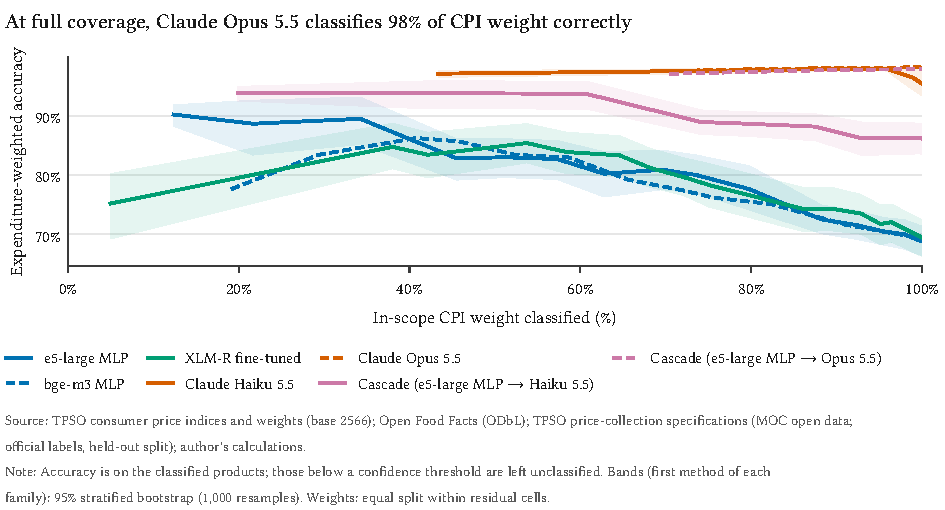
\includegraphics[width=\textwidth]{fig03_frontier.pdf}
\caption{\textbf{At full coverage \NameOpus{} classifies \AccWOpus\% of the evaluated CPI
weight correctly; the cheap methods stay below the LLMs at any coverage.} Weighted accuracy
on the classified products against the in-scope CPI weight classified, as the confidence
threshold rises. Bands (first method of each family): \CfgCI\% stratified bootstrap. Source:
Open Food Facts; MOC; TPSO; author's calculations.}
\label{fig:frontier}
\end{figure}

\paragraph{Where the errors are.} The cheap methods miss whole items. The fine-tuned XLM-R
misses every held-out specification of fresh meat, freshwater fish, processed fish and tobacco
(each a small cell), sends most personal-care specifications to \textsc{oos}, and confuses
seasonings with beverages and cleaning with personal-care products (Figures~\ref{fig:recall}
and~\ref{fig:confusion}); its \NErrXlmrFT{} in-scope errors fall on \NErrSubitemsXlmrFT{}
sub-items. The LLMs' errors are concentrated. \NameOpus's \NErrOpus{} in-scope errors fall on
\NErrSubitemsOpus{} sub-items, and \NErrTopThreeOpus{} of them (\PctErrTopThreeOpus\%) on three;
\NameHaiku's largest three are the same. The TPSO item whose Thai name means ``personal
items'' covers wristwatches, school bags and hair dryers as well as soap and toothpaste. Our
label description, written from the item headings, named only personal-care goods, and both
LLMs sent the held-out wristwatches, school bags and hair dryers to \textsc{oos}. The next
largest error is margarine, which TPSO counts under milk and dairy products and our
description listed under oils and fats; the LLMs followed the description. These are not
failures to read Thai. They are gaps in our documentation of the official item contents, and
they would be closed by better documentation, not by a better model. We did not change the
descriptions after seeing them, since that would tune on the reference set. Because NNLS gives
the personal-items cell a much larger weight than the equal split does, it is this one gap
that lowers the LLM scores under NNLS.

\begin{figure}[t]
\centering
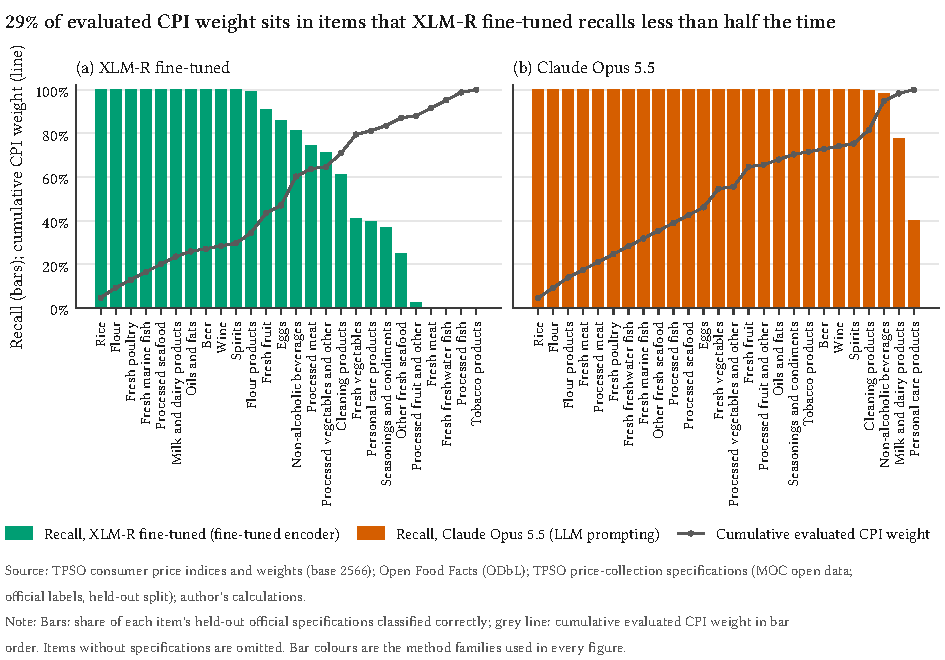
\includegraphics[width=\textwidth]{fig06_item_recall.pdf}
\caption{\textbf{The fine-tuned XLM-R misses whole items; \NameOpus{} misses large parts of
only two.} Recall of each item on the reference set, ranked, with the cumulative in-scope CPI
weight in bar order (line). Items without specifications are omitted. Source: MOC; TPSO;
author's calculations.}
\label{fig:recall}
\end{figure}

\begin{figure}[t]
\centering
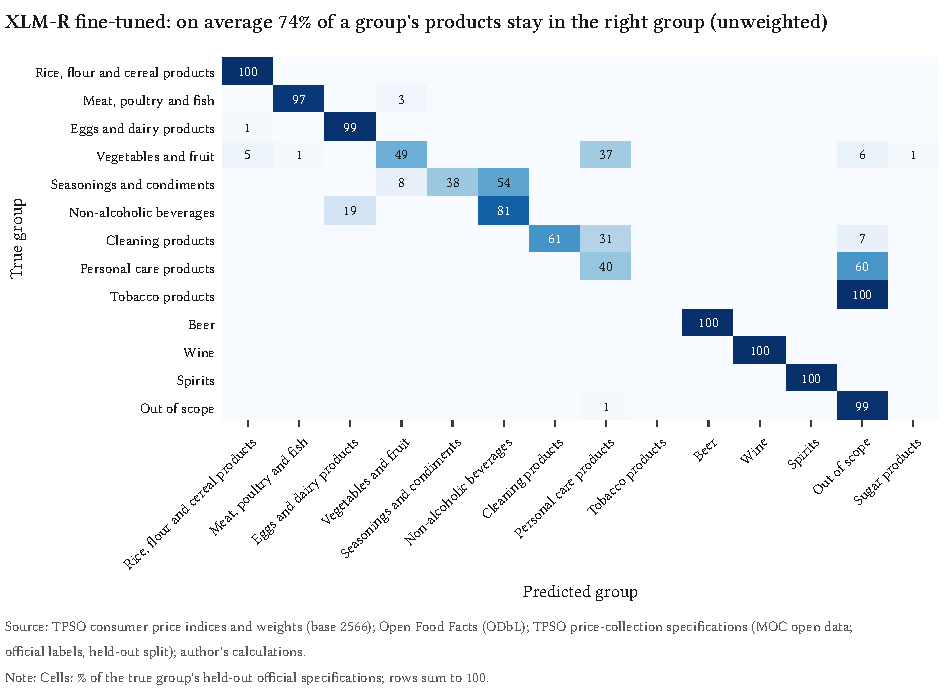
\includegraphics[width=\textwidth]{fig07_group_confusion.pdf}
\caption{\textbf{The best cheap method keeps rice and alcoholic drinks in the right group but
sends tobacco and most personal-care products out of scope and mixes seasonings with beverages
and cleaning with personal-care products.}
Row-normalised confusion between CPI groups for the cheap method with the highest weighted
accuracy (fine-tuned XLM-R); cells are \% of the true group's held-out specifications. Source:
MOC; TPSO; author's calculations.}
\label{fig:confusion}
\end{figure}

\subsection{RQ3: classification error in basis points}\label{sec:rq3}

\textbf{Answer.} With \NameOpus's confusion matrix, measured headline inflation would differ
from official inflation by \BpYoyRmseHeadlineOpus{} basis points (RMSE of the year-on-year
rate, \CfgCI\% interval \BpYoyRmseHeadlineOpusLo--\BpYoyRmseHeadlineOpusHi), food inflation by
\BpYoyRmseFoodOpus{} and core inflation by \BpYoyRmseCoreOpus. With the cheap \NameEfive{} MLP,
the headline error is \BpYoyRmseHeadlineEfiveMLP{} basis points and the food error
\BpYoyRmseFoodEfiveMLP. Accuracy does not rank methods by this error: two cheap methods with
the same weighted accuracy can differ several-fold in basis points.

The simulator covers \NMonthsYoy{} year-on-year rates (\SimFirstYoy{} to \SimLastYoy) and
\NMonthsMom{} month-on-month rates (\SimFirstMom{} to \SimLastMom). Figure~\ref{fig:bp} gives
the year-on-year error of every headline method. Both LLMs and the \NameEfive{}--\NameOpus{}
cascade err by about two to five basis points on every aggregate, with tight intervals; on
month-on-month inflation \NameOpus's headline error is \BpMomRmseHeadlineOpus{} basis points.
For the cheap methods food is where errors bite: \BpYoyRmseFoodEfiveMLP{} basis points for
the \NameEfive{} MLP [\BpYoyRmseFoodEfiveMLPLo, \BpYoyRmseFoodEfiveMLPHi] and
\BpYoyRmseFoodXlmrFT{} for the fine-tuned XLM-R, whose errors are one-sided (a mean of
\BpYoyMeanFoodXlmrFT{} basis points): it understates food inflation in every month
(Figure~\ref{fig:series}). Zero-shot transfer, which RQ1 found to get most of the weight
right, misstates headline inflation by \BpYoyRmseHeadlineEfiveMLPZeroShot{} basis points and
food inflation by \BpYoyRmseFoodEfiveMLPZeroShot{}: getting most of the weight right does not
bound the error from the rest.

\begin{figure}[t]
\centering
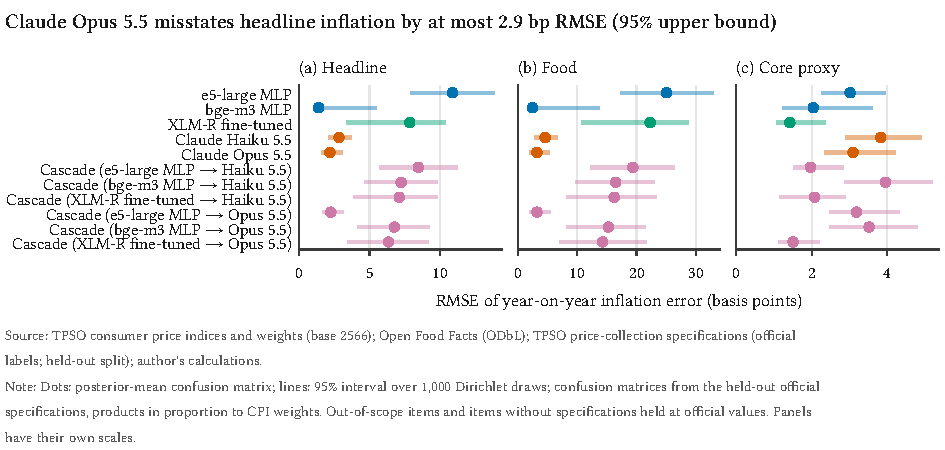
\includegraphics[width=\textwidth]{fig10_bp_error.pdf}
\caption{\textbf{\NameOpus{} misstates headline year-on-year inflation by at most
\BpYoyRmseHeadlineOpusHi{} basis points (RMSE, upper end of the \CfgCI\% interval); every
cheap method's upper end is higher.} RMSE of the year-on-year inflation error over
\NMonthsYoy{} months, headline, food and the core proxy. Dots: posterior-mean confusion matrix;
lines: \CfgCI\% interval over \CfgDraws{} Dirichlet draws. Products in proportion to CPI
weights; out-of-scope items and items without specifications held at official values. Source:
MOC; TPSO; author's calculations.}
\label{fig:bp}
\end{figure}

The \NameBge{} MLP shows why accuracy is not enough. Its weighted accuracy equals the
\NameEfive{} MLP's (\AccWBgeMLP\% against \AccWEfiveMLP\%), but its point estimate of the
headline error is \BpYoyRmseHeadlineBgeMLP{} basis points against \BpYoyRmseHeadlineEfiveMLP.
What matters is not how much weight is misclassified but whether the two items' prices
diverged. The interval for \NameBge{} is wide (\BpYoyRmseHeadlineBgeMLPLo--\BpYoyRmseHeadlineBgeMLPHi)
and the point is at its lower end, so we would not choose a classifier on this point alone. The decomposition of Section~\ref{sec:sim} shows where the
basis points come from (Figure~\ref{fig:decomp}): for the fine-tuned XLM-R, fresh
vegetables classified as fresh fruit contribute more than any other confusion, and
confusions in opposite directions partly cancel. For \NameOpus{} the two largest contributions are
out-of-scope products classified as personal care and margarine counted under oils and fats.
The wristwatches, school bags and hair dryers sent to \textsc{oos} contribute nothing: a
product sent out of scope leaves measurement without entering another item, so in the
simulator it lowers accuracy but adds no bias.

\begin{figure}[t]
\centering
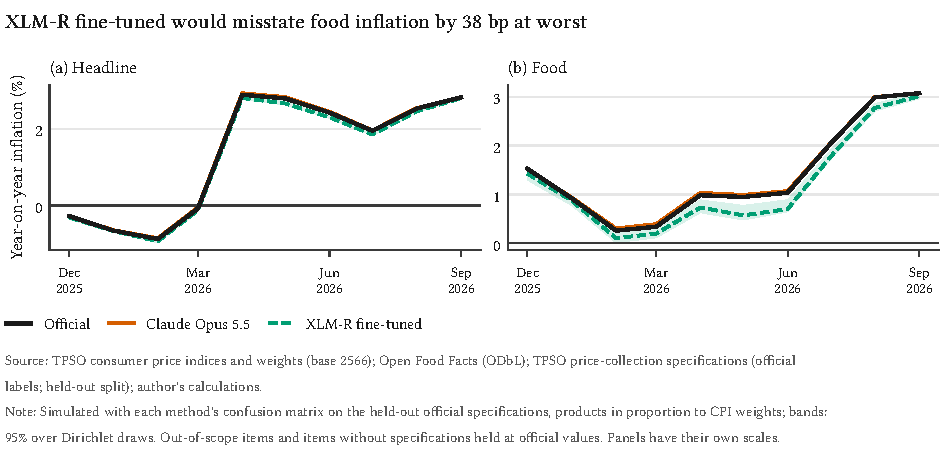
\includegraphics[width=\textwidth]{fig09_series.pdf}
\caption{\textbf{The fine-tuned XLM-R would understate food inflation in every month;
\NameOpus{} tracks the official series.} Official and simulated year-on-year inflation,
headline and food. Bands: \CfgCI\% over Dirichlet draws. Products in proportion to CPI weights.
Source: MOC; TPSO; author's calculations.}
\label{fig:series}
\end{figure}

\begin{figure}[t]
\centering
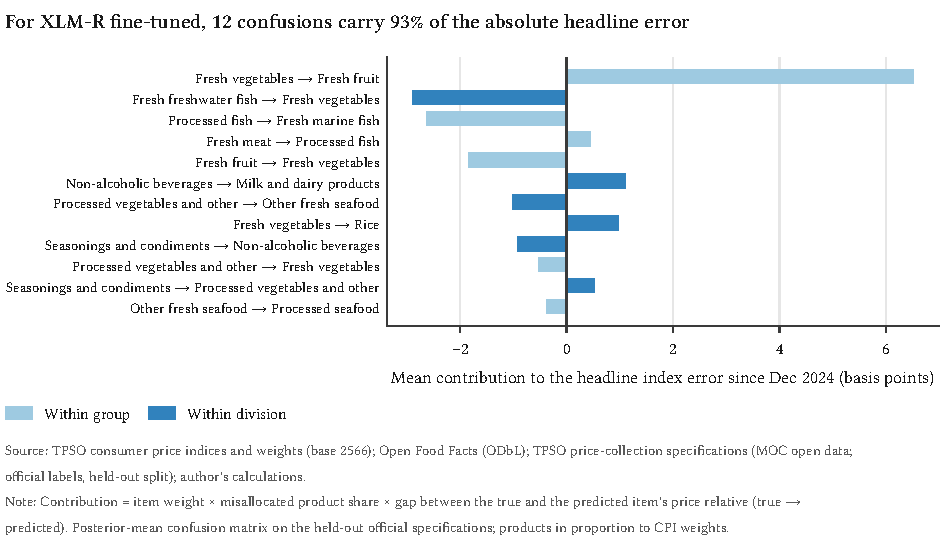
\includegraphics[width=\textwidth]{fig11_where_errors_hurt.pdf}
\caption{\textbf{A handful of confusions carry the headline error of the fine-tuned XLM-R,
and fresh vegetables classified as fresh fruit is the largest.} Mean contribution of each
confusion to the headline index error since the price reference month: item weight times
misallocated product share times the gap between the two items' price relatives. Shade: the
lowest level of the classification the two items share. Source: MOC; TPSO; author's
calculations.}
\label{fig:decomp}
\end{figure}

\paragraph{Robustness.} Three assumptions move these numbers. \emph{The product universe:} if
products arrive in proportion to the office's specification list rather than to CPI weights,
\NameOpus's headline error is \BpYoyRmseHeadlineOpusList{} basis points and the \NameEfive{}
MLP's \BpYoyRmseHeadlineEfiveMLPList. \emph{Product-level noise:} if each product's price
drifts from its item's with an annual standard deviation of \CfgSigmaHi\%, \NameOpus's
headline error rises to \BpYoyRmseHeadlineOpusNoiseTen{} basis points
[\BpYoyRmseHeadlineOpusNoiseTenLo, \BpYoyRmseHeadlineOpusNoiseTenHi], because each item is
then measured from a finite sample of products; at \CfgSigmaLo\% it is \BpYoyRmseHeadlineOpusNoiseFive.
\emph{Coverage alone:} a perfect classifier on the same universe has an error of
\BpYoyRmseHeadlinePerfect{}, so none of the error above comes from the items held at official
values.

\paragraph{Basis points need accuracy alongside.} A product sent out of scope leaves
measurement, and without product-level noise an item measured from a few correctly
classified products is measured exactly. A classifier that sends nearly everything out of
scope therefore looks good in basis points: the \NameEfive{} linear classifier trained on a
hundred official labels alone gets only \AccWEfiveLinMocHundred\% of the weight right, yet its
headline error is \BpYoyRmseHeadlineEfiveLinMocHundred{} basis points. Product-level noise
exposes it: at \CfgSigmaHi\% its error is \BpYoyRmseHeadlineEfiveLinMocHundredNoiseTen{} basis
points, against \BpYoyRmseHeadlineOpusNoiseTen{} for \NameOpus. Neither metric ranks methods
alone; a method should be chosen on both.
